% No new page; first page call under this section. see ProjectStructureSrc . 
\genHeader

\subsection{Your Enterprise Architect Workspace}

Now\hypertarget{projectStructure vis}{} that everything is installed and setup properly, let's take a closer look at the different workspaces and our workflow.
Before we continue, please make a few slight adjustments to Enterprise Architect (EA) so you can easily compare your current workspace to our screenshots.
These settings are advisable but you are, of course, free to choose your own colour schema.

\begin{stepbystep}

\item  Select \menuPath{Tools \menuSep Options \menuSep Themes} in EA, and set Diagram Theme to \texttt{Enterprise Architect 10}.

\item  Next, proceed to \menuPath{Gradients and Background} and set \menuPath{Gradient} and \menuPath{Fill} to \entity{White} (\Cref{ea:paperAndElementFill}). 

\begin{figure}[htbp]
    \centering
    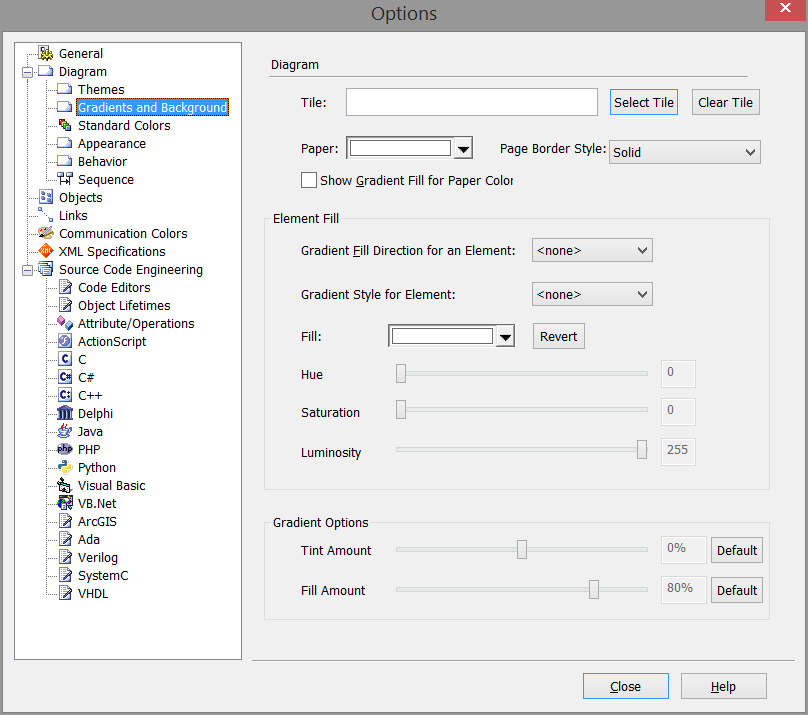
\includegraphics[width=0.8\textwidth]{standardPaperAndFill}
    \caption{Suggested paper background and element fill}
    \label{ea:paperAndElementFill}
\end{figure}

\item  In the \menuPath{Standard Colors} tab, and set your colours to reflect \Cref{ea:standardColoursEA}.

\begin{figure}[htbp]
  \centering
  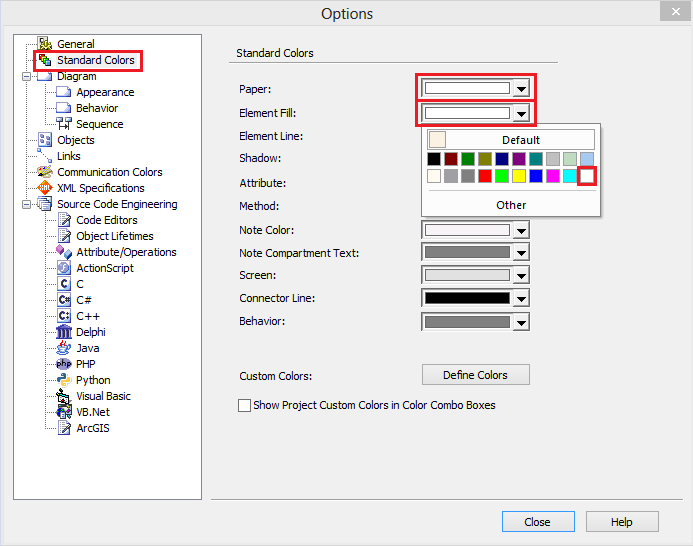
\includegraphics[width=0.8\textwidth]{standardColours}
  \caption{Our choice of standard colours for diagrams in EA}
  \label{ea:standardColoursEA}
\end{figure}

\vspace{0.5cm}

\item 
In the same dialogue, go to \menuPath{Diagram \menuSep Appearance} and reflect the settings in \Cref{ea:standardAppearanceEA}.
Again, this is just a suggestion and not mandatory.

\item 
Last but not least open the \menuPath{Code Engineering} toolbar (\Cref{ea:standardSCEEA1}) and choose \entity{Ecore} as the default language (\Cref{ea:standardSCEEA2}).
\textbf{This setting is mandatory, and very important.}
\end{stepbystep}

\begin{figure}[htbp]
  \centering
  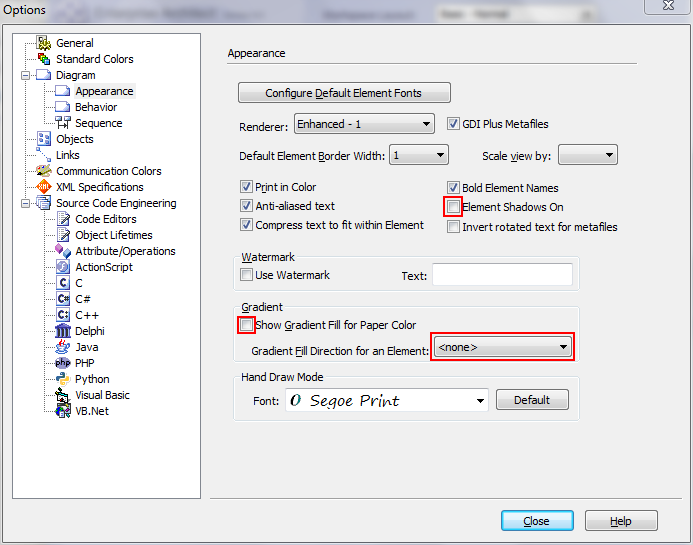
\includegraphics[width=0.8\textwidth]{standardAppearance}
  \caption{Our choice of the standard appearance for model elements}
  \label{ea:standardAppearanceEA}
\end{figure}

\begin{figure}[htbp]
    \centering
    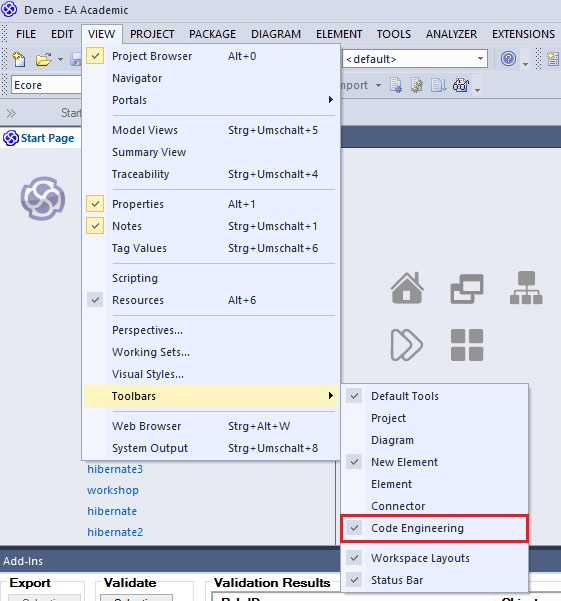
\includegraphics[width=0.8\textwidth]{standardCodeEngineering1}
    \caption{Open the \menuPath{Code Engineering} toolbar}
    \label{ea:standardSCEEA1}
 \end{figure}

\begin{figure}[htbp]
    \centering
    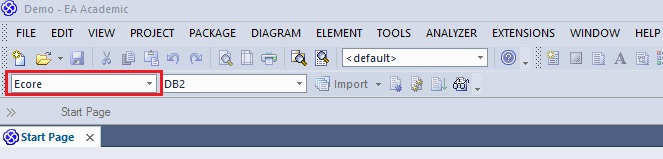
\includegraphics[width=0.8\textwidth]{standardCodeEngineering2}
    \caption{Make sure you set the standard language to \entity{Ecore}}
    \label{ea:standardSCEEA2}
 \end{figure}
 
\clearpage

In your EA \enquote{workspace} (actually referred to as an \emph{EA project}), take a careful look at the project browser:
The root node \texttt{Demo} is called a \emph{model} in EA lingo, and is used as a container to group a set of related \emph{packages}.
In our case, \texttt{Demo} contains a single package \texttt{org.moflon.demo.doublelinkedlist}.
An EA project however, can consist of numerous models that in turn, group numerous packages.

Now switch back to your Eclipse workspace and note the two nodes named \texttt{Specifications} and \texttt{org.moflon.demo} (\Cref{eclipse:eclipsePS}).

\begin{figure}[htbp]
    \centering
    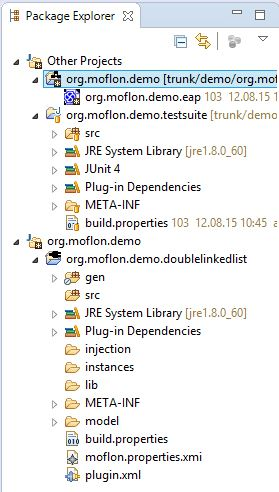
\includegraphics[width=0.4\textwidth]{eclipse_visPackageExplorer}
    \caption{Project structure}
    \label{eclipse:eclipsePS}
 \end{figure}

These nodes, used to group related \emph{Eclipse projects} in an Eclipse workspace, are called \emph{working sets}. The working set
\texttt{Spe\-ci\-fi\-ca\-tions} contains all \emph{metamodel projects} in a  workspace. Your metamodel project contains a single EAP (EA project) file and is
used to communicate with EA and initiate code generation by simply pressing \texttt{F5} or choosing \texttt{Refresh} from the context menu. In our case,
\texttt{Specifications} should contain a single metamodel project \texttt{org.moflon.demo} containing our EA project file \texttt{org.moflon.demo.eap}.
 
\Cref{fig:fromEAtoEclipse} depicts how the Eclipse working set \texttt{org.moflon.demo} and its contents were generated from the EA model \texttt{org.moflon.demo}. Every model
in EA is mapped to a working set in Eclipse with the same name. From every package in the EA model, an Eclipse project is generated, also with the same name.
%\LK{Fix names and screenshot (does not match previous figure)}

\begin{figure}[htbp]
    \centering
  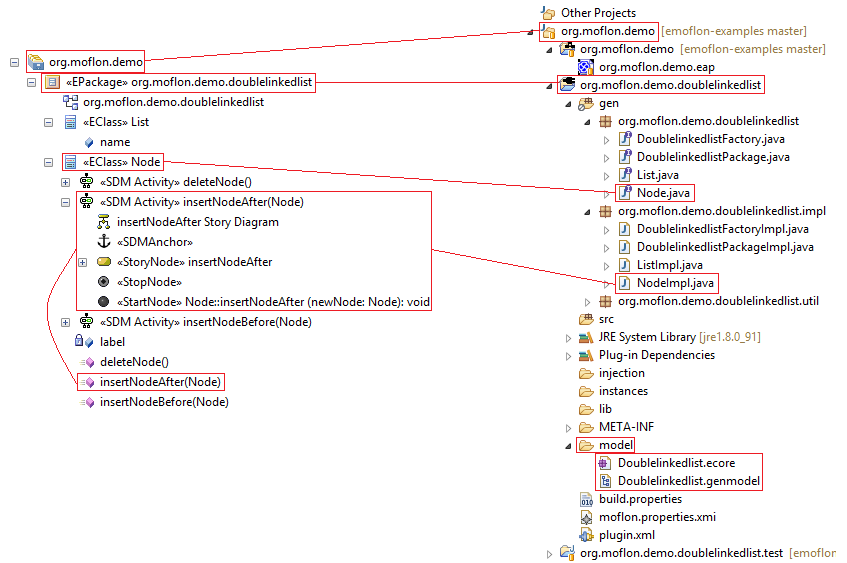
\includegraphics[width=\textwidth]{fromEAToEclipse}
    \caption{Mapping between artefacts in EA and Eclipse}
    \label{fig:fromEAtoEclipse}
\end{figure}

These projects, however, are of a different nature than, for example, metamodel projects or normal Java projects.
These are called \emph{repository projects}.
A \newconcept{nature} is Eclipse lingo for \enquote{project type} and is visually indicated by a corresponding nature icon on the project folder.
Our metamodel projects sport a neat little class diagram symbol.
Repository projects are generated automatically with a certain project structure according to our conventions.

The \entity{model} subfolder in the Eclipse package explorer is probably the most important as it contains the \newconcept{Ecore model} for the project. Ecore is a metamodeling language that provides building blocks such as \newconcept{classes} and \newconcept{references} for defining the static structure (concepts and relations between concepts) of a system.
This folder also contains a \newconcept{genmodel}, the second model required by the Eclipse Modeling Framework (EMF) to generate Java code.

Looking back to \Cref{fig:fromEAtoEclipse}, realize that it also depicts how the class \entity{Node} in the EA model is mapped to the Java interface \entity{Node}.
Double-click \entity{Node.java} and take a look at the methods declared in the interface. These correspond directly to the methods declared in the modeled \entity{Node} class.

As indicated by the source folders \entity{src}, \entity{injection}, and \entity{gen}, we advocate a clean separation of hand-written (should be placed in \entity{src} and \entity{injection}) and generated code (automatically in \texttt{gen}).
As we shall see later in the handbook, hand-written code can be
integrated in generated classes via \emph{injections}.
This is sometimes necessary for small helper functions.

Have you noticed the methods of the \entity{Node} class in our EA model? 
Now hold on tight---each method can be \newconcept{modeled} completely in EA and the corresponding implementation in Java is generated automatically and placed in \texttt{NodeImpl.java}.
Just in case you didn't get it: The behavioural or dynamic aspects of a system can be completely modeled in an abstract, platform-/programming language--independent fashion using a blend of activity diagrams and a \enquote{graph pattern} language called \newconcept{Story~Driven~Modelling}~(SDM).
In our EA project, these \newconcept{Story Diagrams} or simply \emph{SDM}s, are placed in \newconcept{SDM Containers} named according to the method they implement.
For instance, \texttt{\guillemotleft{}SDM Activity\guillemotright{} insertNodeAfter SDM} for the method \texttt{in\-sert\-NodeAft\-er(Node)} as depicted in \Cref{fig:fromEAtoEclipse}.
We'll dedicate Part III of the handbook to understanding why SDMs are so  {\huge crazily} cool!

To recap all we've discussed, let's consider the complete workflow as depicted in \Cref{fig:Overview}. We started with a concise model in EA, simple and
independent of any platform specific details~(1).  Our EA model consists not only of static aspects modelled as a class diagram~(2), but also of dynamic aspects
modelled using SDM~(3).  After exporting the model and code generation~(4), we basically switch from \emph{modelling} to \emph{programming} in a specific
general purpose programming language (Java). On this lower \emph{level of abstraction}, we can flesh out the generated repository~(5) if necessary, and mix as
appropriate with hand-written code and libraries.  Our abstract specification of behaviour (methods) in SDM is translated to a series of method calls that form
the body of the corresponding Java method~(6).

\begin{figure}[htbp]
	\centering
  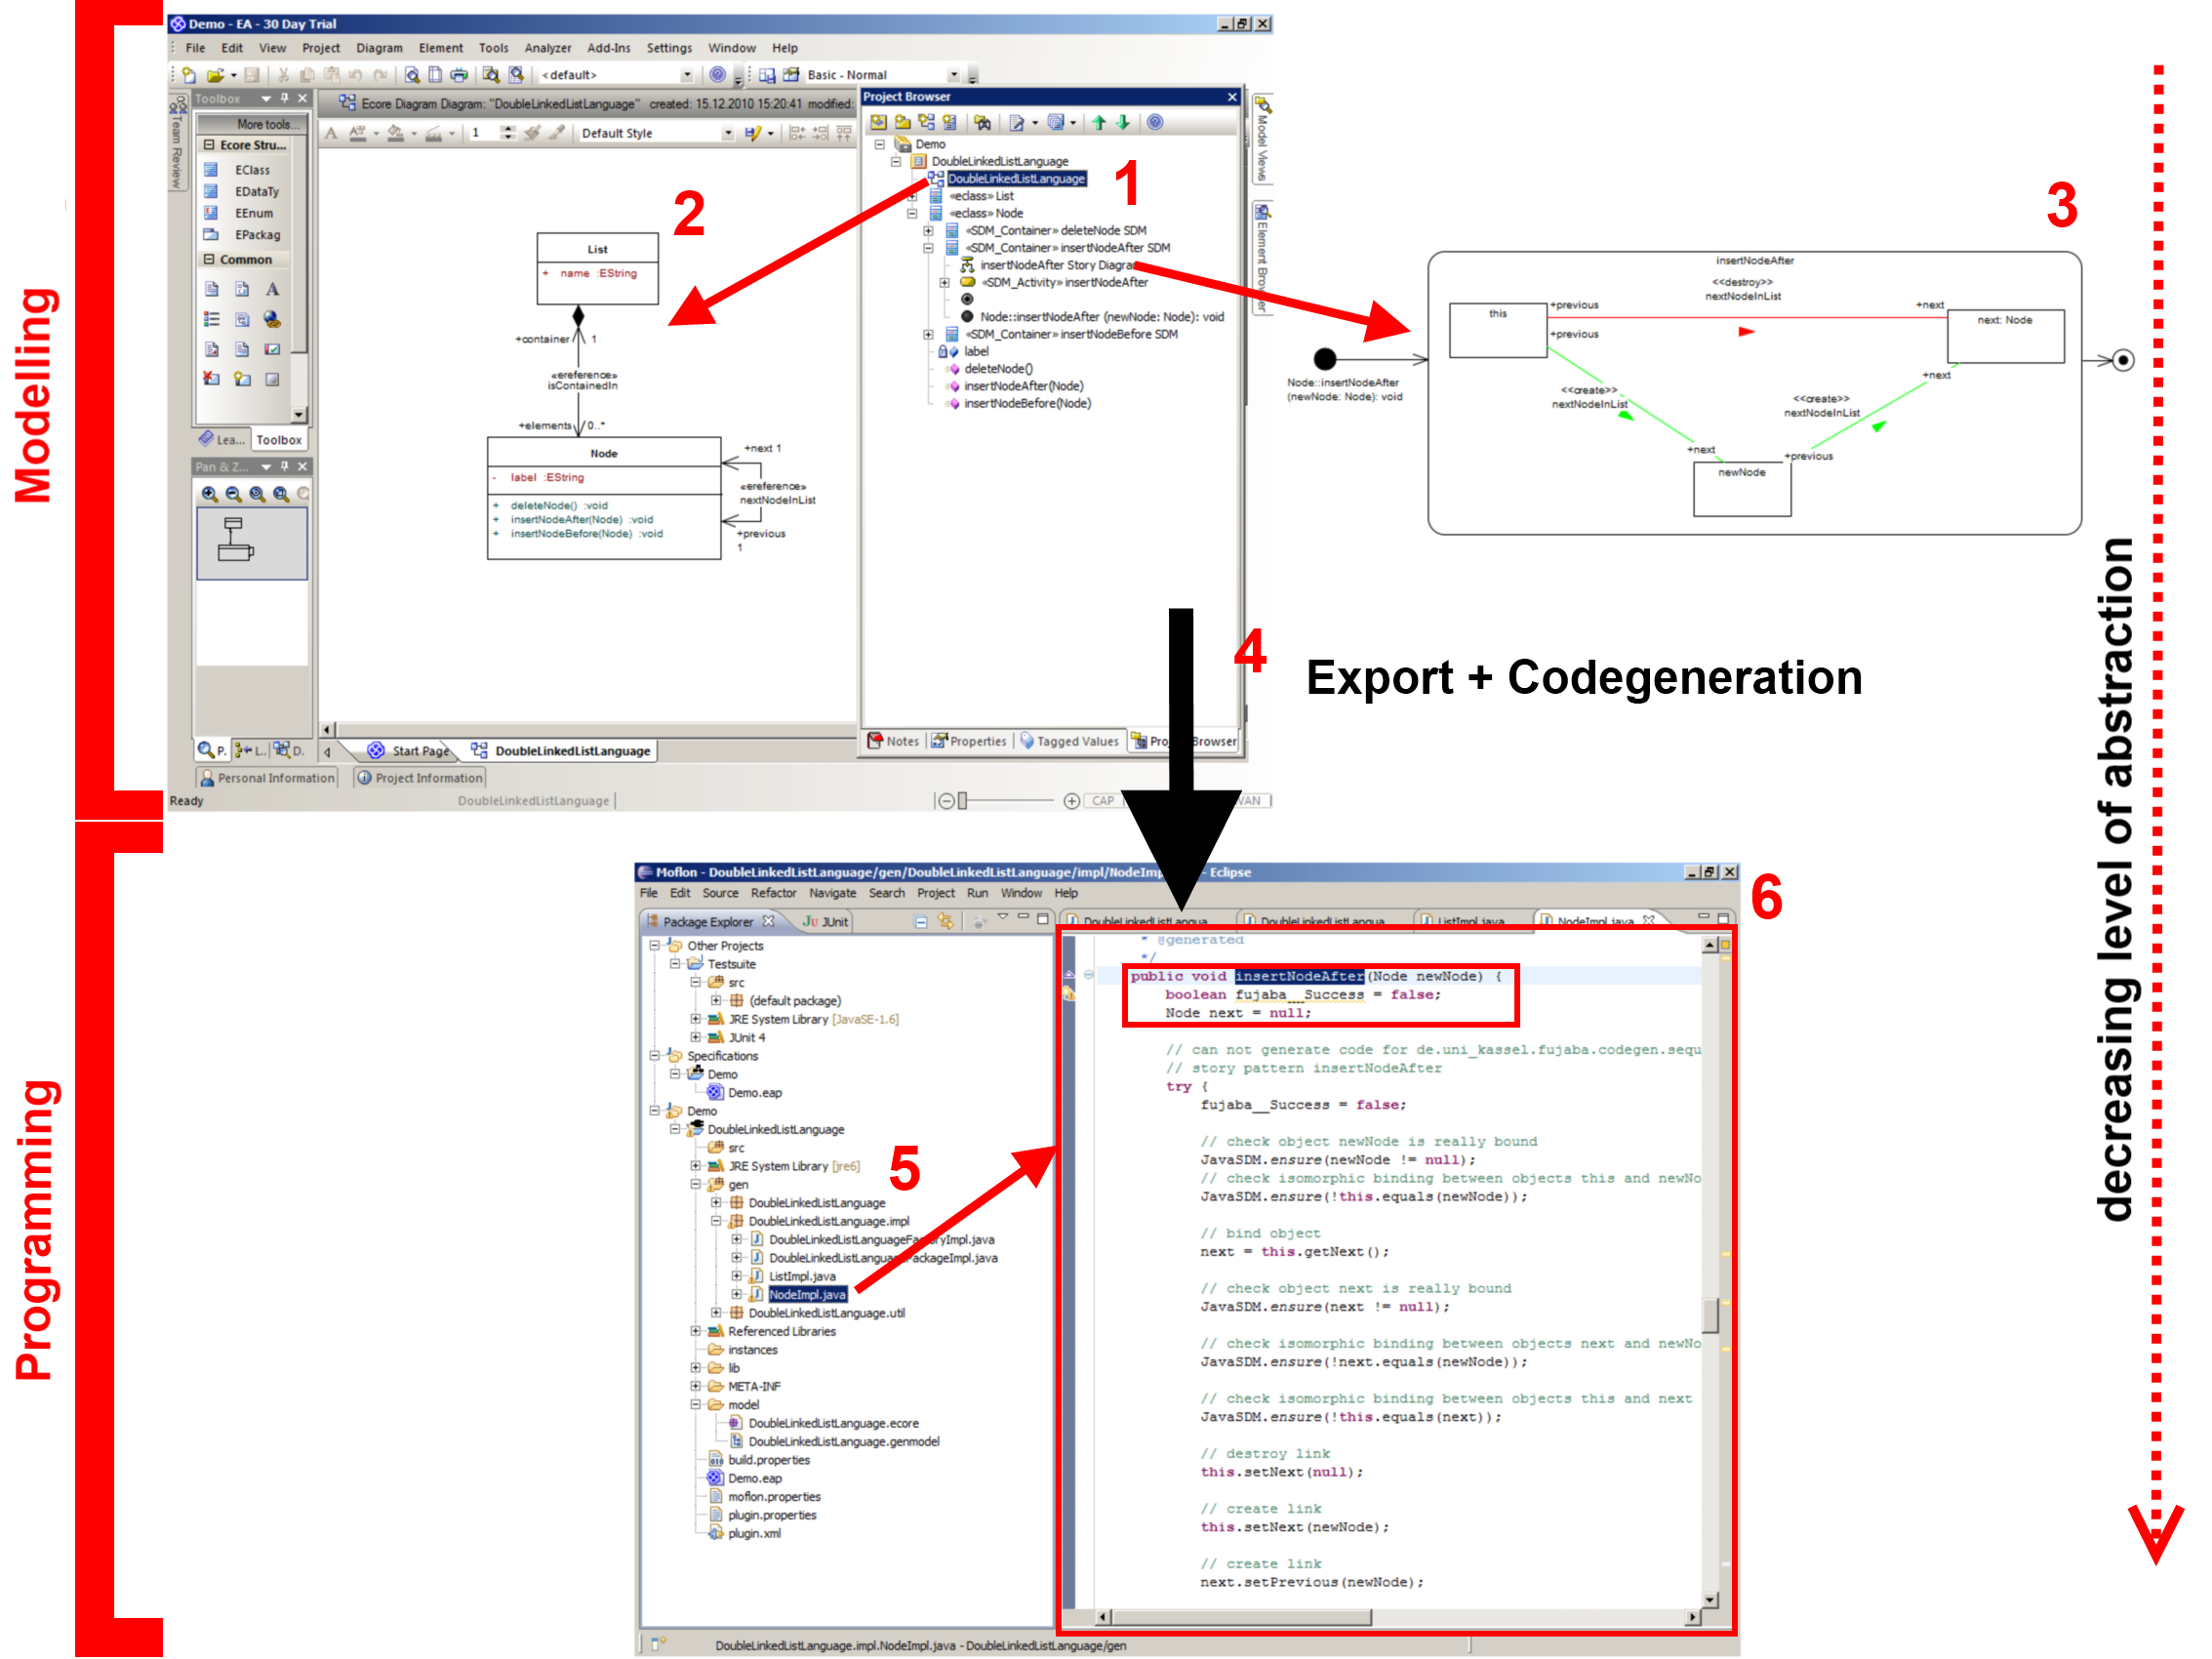
\includegraphics[width=1.1\textwidth]{tafelbild}
	\caption{Overview}
	\label{fig:Overview}
\end{figure}


\clearpage